% Created 2017-05-12 Fri 14:29
% Intended LaTeX compiler: pdflatex
\documentclass[presentation,10pt]{beamer}
\usepackage[utf8]{inputenc}
\usepackage[T1]{fontenc}
\usepackage{graphicx}
\usepackage{grffile}
\usepackage{longtable}
\usepackage{wrapfig}
\usepackage{rotating}
\usepackage[normalem]{ulem}
\usepackage{amsmath}
\usepackage{textcomp}
\usepackage{amssymb}
\usepackage{capt-of}
\usepackage{hyperref}
\usepackage{amsthm}
\usepackage{amsmath}
\usepackage{amssymb}
\usepackage{mathtools}
\newtheorem{mydef}{Definition}
\newtheorem{mythm}{Theorem}
\newcommand{\dx}{\mathrm{d}}
\newcommand{\var}{\mathrm{Var}}
\newcommand{\cov}{\mathrm{Cov}}
\newcommand{\corr}{\mathrm{corr}}
\newcommand{\pr}{\mathrm{Pr}}
\newcommand{\rarrowd}[1]{\xrightarrow{\text{ \textit #1 }}}
\DeclareMathOperator*{\plim}{plim}
\newcommand{\plimn}{\plim_{n \rightarrow \infty}}
\usepackage{booktabs}
\usepackage{color}
\usepackage{caption}
\usepackage{subcaption}
\def\mathbi#1{\textbf{\em #1}}
\setlength{\parskip}{1em}
\usetheme{CambridgeUS}
\usecolortheme{beaver}
\author{Zheng Tian}
\date{}
\title{Lecture 8: Linear Regression with Multiple Regressors}
\hypersetup{
 pdfauthor={Zheng Tian},
 pdftitle={Lecture 8: Linear Regression with Multiple Regressors},
 pdfkeywords={},
 pdfsubject={},
 pdfcreator={Emacs 25.1.1 (Org mode 9.0.3)},
 pdflang={English}}
\begin{document}

\maketitle
\begin{frame}{Outline}
\setcounter{tocdepth}{1}
\tableofcontents
\end{frame}



\section{The Multiple Regression Model}
\label{sec:orgac8874f}
\setcounter{tocdepth}{1}
\tableofcontents[currentsection]

\begin{frame}[label={sec:orgab32b27}]{The problem of a simple linear regression}
\begin{block}{The simple linear regression model}
\begin{equation*}
TestScore = \beta_0 + \beta_1 \times STR + OtherFactors
\end{equation*}
\end{block}

\begin{block}{Question: Is this model adequate to characterize the determination of test scores?}
\begin{itemize}
\item It ignores many important factors, simply lumped into
\emph{OtherFactors}, the error term, \(u_i\), in the regression model.

\item What are possible other important factors?
\begin{itemize}
\item School district characteristics: average income level, demographic
components
\item School characteristics: teachers' quality, school buildings,
\item Student characteristics: family economic conditions, individual
ability
\end{itemize}
\end{itemize}
\end{block}
\end{frame}

\begin{frame}[label={sec:orgc14e700}]{Percentage of English learners as an example}
The percentage of English learners in a school district could be an
relevant and important determinant of test scores, which is omitted
in the simple regression model.

\begin{block}{How can it affect the estimate of the effect of student-teacher ratios on test score?}
\begin{itemize}
\item High percentage of English learners \(\Rightarrow\) large student-teacher ratios.

\item High percentage of English learners \(\Rightarrow\) lower test scores.

\item The estimated effect of student-teacher ratios may in fact include
the influence from the high percentage of English learners.

\item In the terminology of statistics, the magnitude of the coefficient
on student-teacher ratio is \alert{overestimated}.

\item The problem is called \alert{the omitted variable bias}
\end{itemize}
\end{block}
\end{frame}

\begin{frame}[label={sec:org7db03cb}]{Solutions to the problem of ignoring important factors}
We can include these important but ignored variables, like the
percentage of English learners (\(PctEL\)), in the regression model.

\[
TestScore_i = \beta_0 + \beta_1 STR_i + \beta_2 PctEL_i +
OtherFactors_i
\]

A regression model with more than one regressors is a multiple
regression model.
\end{frame}

\begin{frame}[label={sec:org24468b7}]{A multiple regression model}
The general form of a \alert{multiple regression model} is
\begin{equation}
\label{eq:multi-regress-1}
Y_i = \beta_0 + \beta_1 X_{1i} + \beta_2 X_{2i} + \cdots + \beta_k X_{ki} + u_i,\; i = 1, \ldots, n
\end{equation}
where
\begin{itemize}
\item \(Y_i\) is the i\(^{\text{th}}\) observation on the dependent variable;
\item \(X_{1i}, X_{2i}, \ldots, X_{ki}\) are the i\(^{\text{th}}\) observation on each
of the \(k\) regressors; and
\item \(u_i\) is the error term associated with the i\(^{\text{th}}\) observation,
representing all other factors that are not included in the model.
\end{itemize}
\end{frame}

\begin{frame}[label={sec:org45485a7}]{The components in a multiple regression model}
\begin{itemize}
\item The population regression line (or population regression
function)
\begin{equation*}
E(Y_i | X_{1i}, \ldots, X_{ki}) = \beta_0 + \beta_1 X_{1i} + \cdots + \beta_k X_{ki}
\end{equation*}

\item \(\beta_1, \ldots, \beta_k\) are the coefficients on the corresponding
\(X_i,\, i = 1, \ldots, k\).

\item \(\beta_0\) is the intercept, which can also be thought of the
coefficient on a regressor \(X_{0}\) that equals 1 for all
observations.

\begin{itemize}
\item Including \(X_{0}\), there are \(k+1\) regressors in the multiple
regression model.
\end{itemize}
\end{itemize}
\end{frame}

\begin{frame}[label={sec:orgf6292f8}]{The interpretation of \(\beta_i\): Holding other things constant}
\begin{equation}
\label{eq:multi-regress-1a}
Y = \beta_0 + \beta_1 X_1 + \cdots + \beta_k X_k + u
\end{equation}

The coefficient \(\beta_i\) on the regressor
\(X_i\) for \(i=1, \ldots, k\) measures the effect on \(Y\) of a unit change
in \(X_i\), \alert{holding other \(X\) constant}.

\begin{block}{An example}
Suppose we have two regressors \(X_1\) and \(X_2\) and we are interested
in the effect of \(X_1\) on \(Y\). We can let \(X_1\) change by \(\Delta X_1\)
and holding \(X_2\) constant. Then, the new value of \(Y\) is

\[ Y + \Delta Y = \beta_0 + \beta_1 (X_1 + \Delta X_1) + \beta_2 X_2  \]

Subtracting \(Y = \beta_0 + \beta_1 X_1 + \beta_2 X_2\), we have
\(\Delta Y = \beta_1 \Delta X_1\). That is
\[ \beta_1 = \frac{\Delta Y}{\Delta X}, \text{ holding } X_2 \text{ constant} \]
\end{block}
\end{frame}

\begin{frame}[label={sec:org22b307e}]{The partial effect}
If \(Y\) and \(X_i\) for \(i = 1, \ldots, k\) are continuous and
differentiable variables, \(\beta_i\) is as simply as the partial
derivative of \(Y\) with respect to \(X_i\). That is

\[\beta_i = \frac{\partial Y}{\partial X_i}\]

By the definition of a partial derivative, \(\beta_i\) is just
the effect of a marginal change in \(X_i\) on \(Y\) holding other \(X\)
constant.
\end{frame}

\begin{frame}[label={sec:org1af89e4}]{Look at the data in terms of vectors and matrix}
\begin{figure}[htbp]
\centering
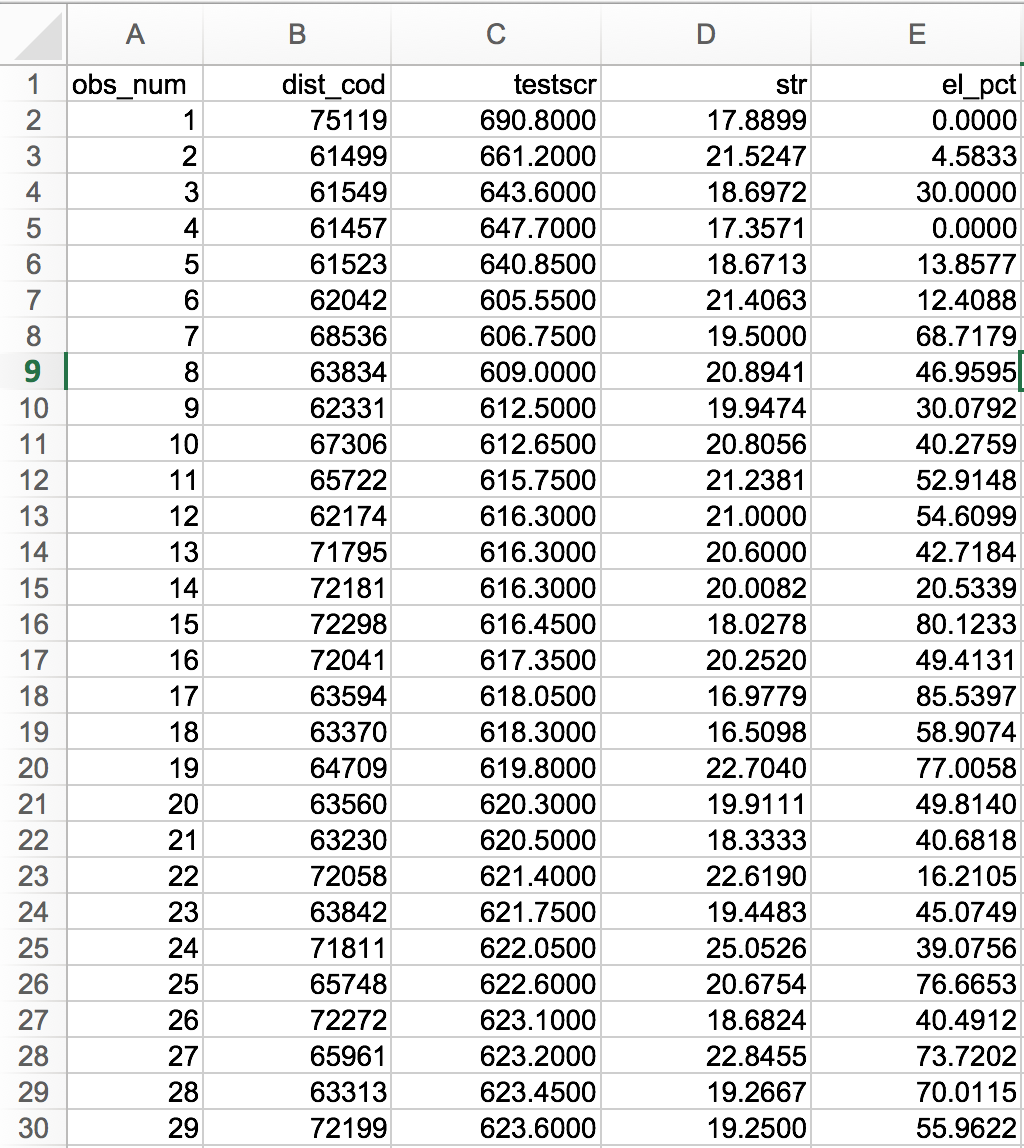
\includegraphics[width=0.4\textwidth,height=0.5\textheight]{img/data_snapshot.png}
\caption{\label{fig:orgb79c74a}
The California data set in Excel}
\end{figure}

\begin{itemize}
\item Each row represents an observation of all variables pertaining to a
school district.
\item Each column represents a variable with all
observations.
\item The whole dataset can be seen as a matrix.
\end{itemize}
\end{frame}

\begin{frame}[shrink,label={sec:org2ba62ad}]{Define variables in matrix notation}
\begin{block}{Write all the variables in vector and matrix notation}
\begin{equation*}
\underbrace{
\mathbf{Y} =
\begin{pmatrix}
Y_1 \\
Y_2 \\
\vdots \\
Y_n
\end{pmatrix},}_{\text{Dependent variable}}
\underbrace{
\mathbf{X} =
\begin{pmatrix}
1 & X_{11} & \cdots & X_{k1} \\
1 & X_{12} & \cdots & X_{k2} \\
\vdots & \vdots & \ddots & \vdots \\
1 & X_{1n} & \cdots & X_{kn}
\end{pmatrix},}_{\text{Independent variables}}
\underbrace{
\mathbf{u} =
\begin{pmatrix}
u_1 \\
u_2 \\
\vdots \\
u_n
\end{pmatrix},\,}_{\text{Errors}}
\underbrace{
\boldsymbol{\beta} =
\begin{pmatrix}
\beta_0 \\
\beta_1 \\
\vdots \\
\beta_k
\end{pmatrix}}_{\text{Coefficients}}
\end{equation*}
\end{block}

\begin{block}{Write the multiple regression model in matrix notation}
\begin{equation}
\label{eq:multi-regress-m}
\mathbf{Y} = \mathbf{X} \boldsymbol{\beta} + \mathbf{u}
\end{equation}
\end{block}

\begin{block}{Why do we use matrix notation}
Concise, easy to derive properties; big-picture perspective.
\end{block}
\end{frame}


\begin{frame}[label={sec:org5fd6870}]{Two other ways to write the regression model}
\begin{block}{Write \(\mathrm{X}\) in row vectors}
\begin{itemize}
\item The i\(^{\text{th}}\) row in \(\mathrm{X}\) is a \((k+1) \times 1\) vector
\begin{equation*}
\mathbi{x}_i =
\begin{pmatrix}
1 \\
X_{1i} \\
\vdots \\
X_{ki} \\
\end{pmatrix}. \text{ Thus, its transpose is }
\mathbi{x}_i^{\prime} = (1, X_{1i}, \cdots, X_{ki})
\end{equation*}

\item We can write the regression model (Equation
\ref{eq:multi-regress-m}) as

\begin{equation}
Y_i = \mathbi{x}^{\prime}_i \boldsymbol{\beta} + u_i,\; i = 1, \ldots, n
\end{equation}
\end{itemize}
\end{block}
\end{frame}

\begin{frame}[label={sec:org82c6e63}]{Two other ways to write the regression model (cont'd)}
\begin{block}{Write \(\mathrm{X}\) in vector vectors}
\begin{itemize}
\item The i\(^{\text{th}}\) column in \(\mathbf{X}\) is a \(n \times 1\) vector
\begin{equation*}
\boldsymbol{X}_i =
\begin{pmatrix}
X_{i1} \\
\vdots \\
X_{in} \\
\end{pmatrix}. \text{ The first column is }
\boldsymbol{\iota} =
\begin{pmatrix}
1 \\
\vdots \\
1
\end{pmatrix}. \text{ Thus }
\mathbf{X} = \left(\boldsymbol{\iota}, \boldsymbol{X}_1, \ldots, \boldsymbol{X}_k \right)
\end{equation*}

\item The regression model (Equation \ref{eq:multi-regress-m}) can be
re-written as
\begin{equation}
\label{eq:multi-regress-m2}
\mathbf{Y} = \beta_0 \boldsymbol{\iota} + \beta_1\boldsymbol{X}_1 + \cdots + \beta_k\boldsymbol{X}_k + \mathbf{u}
\end{equation}
\end{itemize}
\end{block}
\end{frame}


\section{The OLS Estimator in Multiple Regression}
\label{sec:org8975730}
\setcounter{tocdepth}{1}
\tableofcontents[currentsection]

\begin{frame}[label={sec:org18c0f27}]{The minimization problem and the OLS estimator}
\begin{itemize}
\item The core idea of the OLS estimator for a multiple regression model
remains the same as in a simple regression model:
\alert{minimizing the sum of the squared residuals}.

\item Let \(\mathbf{b} = [b_0, b_1, \ldots, b_k]^{\prime}\) be some estimators
of \(\boldsymbol{\beta} = [\beta_0, \beta_1, \ldots,
  \beta_k]^{\prime}\).

\item The predicted \(Y_i\) is
\begin{gather*}
\hat{Y}_i = b_0 + b_1 X_{1i} + \cdots + b_k X_{ki} = \mathbi{x}^{\prime}_i
\mathbf{b},\, i = 1, \ldots, \\
\text{ or in matrix notation }  \hat{\mathbf{Y}} = \mathbf{Xb}
\end{gather*}

\item The residuals, i.e., the prediction mistakes, with \(\mathbf{b}\) is
\begin{gather*}
\hat{u}_i = Y_i - b_0 - b_1 X_{1i} - \cdots - b_k X_{ki} = Y_i -
\mathbi{x}^{\prime}_i \mathbf{b} \\
\text{ or in matrix notation }  \hat{\mathbf{u}} = \mathbf{Y} - \mathbf{Xb}
\end{gather*}
\end{itemize}
\end{frame}

\begin{frame}[label={sec:orgf5f867b}]{The minimization problem and the OLS estimator (cont'd)}
\begin{itemize}
\item The sum of the squared residuals is
\begin{align*}
S(\mathbf{b}) & = S(b_0, b_1, \ldots, b_k) = \sum_{i=1}^n (Y_i - b_0 - b_1 X_{1i} - \cdots - b_k X_{ki})^2 \\
& = \sum_{i=1}^n (Y_i - \mathbf{x}^{\prime}_i \mathbf{b})^2 = (\mathbf{Y} -
\mathbf{Xb})^{\prime}(\mathbf{Y}-\mathbf{Xb}) \\
& = \hat{\mathbf{u}}^{\prime} \hat{\mathbf{u}} = \sum_{i=1}^n \hat{u}_i^2
\end{align*}

\item The OLS estimator is the solution to the following minimization problem:
\begin{equation}
\label{eq:ols-multi-regress}
\operatorname*{min}_{\mathbf{b}}\: S(\mathbf{b}) = \hat{\mathbf{u}}^{\prime} \hat{\mathbf{u}}
\end{equation}
\end{itemize}
\end{frame}

\begin{frame}[label={sec:orgbf71406}]{The OLS estimator of \(\boldsymbol{\beta}\) as a solution to the minimization problem}
\begin{itemize}
\item Solve the minimization problem:

$$\text{F.O.C.: } \frac{\partial S(\mathbf{b})}{\partial b_j} = 0,
  \text{ for } j =
  0, 1, \ldots, k$$

\item The derivative of \(S(b_0, \ldots, b_k)\) with respect to \(b_j\) is
\begin{gather*}
\label{eq:ols-wrt-bj}
\frac{\partial }{\partial b_j} \sum_{i=1}^n \left(Y_i - b_0 - b_1 X_{1i} - \cdots - b_k X_{ki} \right)^2 = \\
-2 \sum_{i=1}^n X_{ji} \left(Y_i - b_0 - b_1 X_{1i} - \cdots - b_k X_{ki} \right) = 0
\end{gather*}

\item There are \(k+1\) such equations. Solving the system of equations, we
obtain the OLS estimator \(\hat{\boldsymbol{\beta}} = (\hat{\beta}_0, \ldots,
  \hat{\beta}_k)^{\prime}\).
\end{itemize}
\end{frame}

\begin{frame}[label={sec:org015d47d}]{The OLS estimator in matrix notation}
Let \(\boldsymbol{\hat{\beta}}\) denote the OLS estimator. Then the
expression of \(\boldsymbol{\hat{\beta}}\) is given by
\begin{equation}
\label{eq:betahat-mult}
\boldsymbol{\hat{\beta}} = (\mathbf{X}^{\prime} \mathbf{X})^{-1} \mathbf{X}^{\prime} \mathbf{Y}
\end{equation}

\begin{block}{Some useful results of matrix calculus}
To prove Equation (\ref{eq:betahat-mult}), we need to use some results
of matrix calculus.
\begin{equation}
\label{eq:matrix-calc}
\frac{\partial \mathbf{a}^{\prime} \mathbf{x}}{\partial \mathbf{x}} = \mathbf{a},\; \frac{\partial \mathbf{x}^{\prime} \mathbf{a}}{\partial \mathbf{x}} = \mathbf{a},\; \text{ and } \frac{\partial \mathbf{x}^{\prime} \mathbf{A} \mathbf{x}}{\partial \mathbf{x}} = (\mathbf{A} + \mathbf{A}^{\prime}) \mathbf{x}
\end{equation}
when \(\mathbf{A}\) is symmetric, then \((\partial \mathbf{x}^{\prime}
\mathbf{A} \mathbf{x}) / (\partial \mathbf{x}) = 2\mathbf{A}
\mathbf{x}\)
\end{block}
\end{frame}

\begin{frame}[label={sec:orgc08e9e0}]{The proof}
\begin{proof}[Proof of Equation (\ref{eq:betahat-mult})]
  \begin{equation*}
  S(\mathbf{b}) = \hat{\mathbf{u}}^{\prime} \hat{\mathbf{u}} = \mathbf{Y}^{\prime} \mathbf{Y} - \mathbf{b}^{\prime} \mathbf{X}^{\prime} \mathbf{Y} - \mathbf{Y}^{\prime} \mathbf{Xb} - \mathbf{b}^{\prime} \mathbf{X}^{\prime} \mathbf{Xb}
  \end{equation*}

  The first order conditions for minimizing $S(\mathbf{b})$ with respect to $\mathbf{b}$ is
  \begin{gather}
  -2 \mathbf{X}^{\prime} \mathbf{Y} - 2 \mathbf{X}^{\prime} \mathbf{Xb} = \mathbf{0} \notag \\
  \mathbf{X}^{\prime} \mathbf{Xb} = \mathbf{X}^{\prime} \mathbf{Y} \label{eq:ols-mult-eqs}
  \end{gather}

  Then
  \begin{equation*}
  \mathbf{b} = (\mathbf{X}^{\prime} \mathbf{X})^{-1} \mathbf{X}^{\prime} \mathbf{Y}
  \end{equation*}
  given that $\mathbf{X}^{\prime} \mathbf{X}$ is invertible.
\end{proof}

Note that Equation (\ref{eq:ols-mult-eqs}) represents a system of
equations with \(k+1\) equations.
\end{frame}

\begin{frame}[label={sec:org21c24be}]{The OLS estimator of \(\hat{\beta}_1\) in a simple regression model}
The simple linear regression model written in matrix notation is

\begin{equation*}
\mathbf{Y} = \beta_0 \boldsymbol{\iota} + \beta_1 \mathbf{X}_1 + \mathbf{u} = \mathbf{X} \boldsymbol{\beta} + \mathbf{u}
\end{equation*}

where

\begin{equation*}
\mathbf{Y} =
\begin{pmatrix}
Y_1 \\
\vdots \\
Y_n
\end{pmatrix},\,
\mathbf{X} =
\begin{pmatrix}
\boldsymbol{\iota} & \mathbf{X}_1
\end{pmatrix}
=
\begin{pmatrix}
1 & X_{11} \\
\vdots & \vdots \\
1 & X_{1n}
\end{pmatrix},\,
\mathbf{u} =
\begin{pmatrix}
u_1 \\
\vdots \\
u_n
\end{pmatrix},\,
\boldsymbol{\beta} =
\begin{pmatrix}
\beta_0 \\
\beta_1 \\
\end{pmatrix}
\end{equation*}
\end{frame}

\begin{frame}[plain,label={sec:orgd9df225}]{The OLS estimator of \(\hat{\beta}_1\) in a simple regression model (cont'd)}
Let's get the components in Equation (\ref{eq:betahat-mult}) step by
step.

\begin{block}{Step (1): compute \(\left(\mathbf{X}^{\prime}\mathbf{X}\right)\)}
\begin{align*}
\mathbf{X}^{\prime}\mathbf{X} & =
\begin{pmatrix}
\boldsymbol{\iota}^{\prime} \\
\mathbf{X}_1^{\prime}
\end{pmatrix}
\begin{pmatrix}
\boldsymbol{\iota} & \mathbf{X}_1
\end{pmatrix} =
\begin{pmatrix}
1 & \cdots & 1 \\
X_{11} & \cdots & X_{1n}
\end{pmatrix}
\begin{pmatrix}
1 & X_{11} \\
\vdots & \vdots \\
1 & X_{1n}
\end{pmatrix} \\
& =
\begin{pmatrix}
\boldsymbol{\iota}^{\prime} \boldsymbol{\iota} & \boldsymbol{\iota}^{\prime} \mathbf{X}_1 \\
\mathbf{X}_1^{\prime} \boldsymbol{\iota} & \mathbf{X}_1^{\prime} \mathbf{X}_1
\end{pmatrix} =
\begin{pmatrix}
n & \sum_{i=1}^n X_{1i} \\
\sum_{i=1}^n X_{1i} & \sum_{i=1}^n X_{1i}^2
\end{pmatrix}
\end{align*}
\end{block}
\end{frame}

\begin{frame}[plain,label={sec:orgc40898b}]{The OLS estimator of \(\hat{\beta}_1\) in a simple regression model (cont'd)}
\begin{description}
\item[{Step (2): compute \(\left(\mathbf{X}^{\prime}\mathbf{X}\right)^{-1}\)}]
\end{description}

\begin{block}{The inverse of a \(2 \times 2\) matrix}
\begin{equation*}
\begin{pmatrix}
a_{11} & a_{12} \\
a_{21} & a_{22}
\end{pmatrix}^{-1}
=\frac{1}{a_{11}a_{22} - a_{12}a_{21}}
\begin{pmatrix}
a_{22} & -a_{12} \\
-a_{21} & a_{11}
\end{pmatrix}
\end{equation*}
\end{block}

\begin{block}{The inverse of \(\mathbf{X}^{\prime}\mathbf{X}\)}
\begin{equation*}
\left(\mathbf{X}^{\prime}\mathbf{X}\right)^{-1} =
\frac{1}{n \sum_{i=1}^n X_{1i}^2 - (\sum_{i=1}^n X_{1i})^2}
\begin{pmatrix}
\sum_{i=1}^n X_{1i}^2 & - \sum_{i=1}^n X_{1i} \\
-\sum_{i=1}^n X_{1i} & n
\end{pmatrix}
\end{equation*}
\end{block}
\end{frame}

\begin{frame}[plain,label={sec:org1fa8bb1}]{The OLS estimator of \(\hat{\beta}_1\) in a simple regression model (cont'd)}
\begin{block}{Step (3): compute \(\mathbf{X}^{\prime} \mathbf{Y}\)}
\begin{equation*}
\mathbf{X}^{\prime} \mathbf{Y} =
\begin{pmatrix}
\boldsymbol{\iota}^{\prime} \\
\mathbf{X}_1^{\prime}
\end{pmatrix}
\mathbf{Y} =
\begin{pmatrix}
1 & \cdots & 1 \\
X_{11} & \cdots & X_{1n}
\end{pmatrix}
\begin{pmatrix}
Y_1 \\
\vdots \\
Y_n
\end{pmatrix} =
\begin{pmatrix}
\boldsymbol{\iota}^{\prime} \mathbf{Y} \\
\mathbf{X}_1^{\prime} \mathbf{Y}
\end{pmatrix} =
\begin{pmatrix}
\sum_{i=1}^n Y_i \\
\sum_{i=1}^n X_{1i} Y_i
\end{pmatrix}
\end{equation*}
\end{block}

\begin{block}{Step (4): compute \(\boldsymbol{\hat{\beta}}=(\mathbf{X}^{\prime}\mathbf{X})^{-1} \mathbf{X}^{\prime} \mathbf{Y}\)}
\begin{align*}
\begin{pmatrix}
\hat{\beta}_0 \\
\hat{\beta}_1
\end{pmatrix} & =
\frac{1}{n \sum_{i=1}^n X_{1i}^2 - (\sum_{i=1}^n X_{1i})^2}
\begin{pmatrix}
\sum_{i=1}^n X_{1i}^2 & - \sum_{i=1}^n X_{1i} \\
-\sum_{i=1}^n X_{1i} & n
\end{pmatrix}
\begin{pmatrix}
\sum_{i=1}^n Y_i \\
\sum_{i=1}^n X_{1i} Y_i
\end{pmatrix} \\
& =
\frac{1}{n \sum_{i=1}^n X_{1i}^2 - (\sum_{i=1}^n X_{1i})^2}
\begin{pmatrix}
\sum_{i=1}^n X_{1i}^2 \sum_{i=1}^n Y_i - \sum_{i=1}^n X_{1i} \sum_{i=1}^n X_{1i}Y_i \\
-\sum_{i=1}^n X_{1i} \sum_{i=1}^n Y_i + n \sum_{i=1}^n X_{1i} Y_i
\end{pmatrix}
\end{align*}
\end{block}
\end{frame}

\begin{frame}[plain,label={sec:orgcf791c6}]{The OLS estimator of \(\hat{\beta}_1\) in a simple regression model (cont'd)}
\begin{block}{The formula of \(\hat{\beta}_1\)}
\begin{equation*}
\hat{\beta}_1 = \frac{n \sum_{i=1}^n X_{1i} Y_i - \sum_{i=1}^n X_{1i} \sum_{i=1}^n Y_i}{n \sum_{i=1}^n X_{1i}^2 - (\sum_{i=1}^n X_{1i})^2} = \frac{\sum_{i=1}^n (X_{1i} - \bar{X}_1)(Y_i - \bar{Y})}{\sum_{i=1}^n (X_{1i} - \bar{X}_1)^2}
\end{equation*}
\end{block}

\begin{block}{The formula of \(\hat{\beta}_0\)}
\begin{equation*}
\hat{\beta}_0 = \frac{\sum_{i=1}^n X_{1i}^2 \sum_{i=1}^n Y_i - \sum_{i=1}^n X_{1i} \sum_{i=1}^n X_{1i}Y_i}{n \sum_{i=1}^n X_{1i}^2 - (\sum_{i=1}^n X_{1i})^2} = \bar{Y} - \hat{\beta}_1 \bar{X}_1
\end{equation*}
\end{block}
\end{frame}

\begin{frame}[shrink,plain,label={sec:orge9b07b4}]{Application to Test Scores and the Student-Teacher Ratio}
\begin{block}{The simple regression compared with the multiple regression}
The estimated simple linear regression model is
\[ \widehat{TestScore} = 698.9 - 2.28 \times STR \]

The estimated multiple linear regression model is
\[ \widehat{TestScore} = 686.0 - 1.10 \times STR - 0.65 \times PctEL
\]
\end{block}

\begin{block}{Explanations}
\begin{itemize}
\item The interpretation of the new estimated coefficient on \emph{STR} is,
\alert{holding the percentage of English learners constant}, a unit
decrease in \emph{STR} is estimated to increase test scores by 1.10
points.
\item We can also interpret the estimated coefficient on \emph{PctEL} as,
holding \emph{STR} constant, one unit decrease in \emph{PctEL} increases test
scores by 0.65 point.
\item The magnitude of the negative effect of \emph{STR} on test scores in the
multiple regression is approximately half as large as when \emph{STR} is
the only regressor.
\end{itemize}
\end{block}
\end{frame}

\begin{frame}[shrink,label={sec:org45b57cb}]{Warm-up exercises}
\begin{block}{1) In the multiple regression model you estimate the effect on Yi of a unit change in one of the Xi while holding all other regressors constant. This}
\begin{description}
\item[{A)}] makes little sense, because in the real world all other variables change.
\item[{B)}] corresponds to the economic principle of mutatis mutandis.
\item[{C)}] leaves the formula for the coefficient in the single explanatory variable case unaffected.
\item[{D)}] corresponds to taking a partial derivative in mathematics.
\end{description}
\pause
Answer:  D
\end{block}

\begin{block}{2) The multiple regression model can be written in matrix form as follows:}
\begin{description}
\item[{A)}] \(\mathbf{Y} = \mathbf{X} \boldsymbol{\beta}\)
\item[{B)}] \(\mathbf{Y} = \mathbf{X} + \mathbf{U}\)
\item[{C)}] \(\mathbf{Y} = \boldsymbol{\beta} \mathbf{X} + \mathbf{U}\)
\item[{D)}] \(\mathbf{Y} = \mathbf{X} \boldsymbol{\beta} + \mathbf{U}\)
\end{description}
\pause
Answer:  D
\end{block}

\begin{block}{3) Minimization of \(\sum_{i=1}^n (Y_i - b_0 - b_1 X_{1i} - \cdots - b_k X_{ki})^2\) results in}
\begin{description}
\item[{A)}] \(\mathbf{X}^{\prime}\mathbf{Y} = \mathbf{X} \hat{\boldsymbol{\beta}}\)
\item[{B)}] \(\mathbf{X} \hat{\boldsymbol{\beta}} = \mathbf{0}_{k+1}\)
\item[{C)}] \(\mathbf{X}^{\prime} (\mathbf{Y} - \mathbf{X} \hat{\boldsymbol{\beta}}) = \mathbf{0}_{k+1}\)
\item[{D)}] \(\mathbf{R} \boldsymbol{\beta} = \mathbf{r}\)
\end{description}
\pause
Answer:  C
\end{block}
\end{frame}


\section{Measures of Fit in Multiple Regression}
\label{sec:orgf9653bd}
\setcounter{tocdepth}{1}
\tableofcontents[currentsection]

\begin{frame}[label={sec:org241d2cb}]{The standard errors of the regression (SER)}
\begin{itemize}
\item The standard error of regression (SER) estimates the standard
deviation of the error term \(\mathbf{u}\). In multiple regression,
the SER is
\begin{equation}
\label{eq:ser-m}
SER = s_{\hat{u}},\, \text{ where } s^2_{\hat{u}} = \frac{\sum_{i=1}^n \hat{u}_i^2}{n-k-1} = \frac{SSR}{n-k-1}
\end{equation}

\item \(SSR\) is divided by \((n-k-1)\) because there are \(n\) observations and
\((k+1)\) coefficients to be estimated.
\end{itemize}
\end{frame}

\begin{frame}[label={sec:orgdf814bd}]{\(R^2\)}
\begin{block}{TSS, ESS, and SSR}
\begin{itemize}
\item The total sum of squares (TSS): \(TSS = \sum_{i=1}^n (Y_i - \bar{Y})^2\)
\item The explained sum of squares (ESS): \(ESS = \sum_{i=1}^n (\hat{Y}_i - \bar{Y})^2\)
\item The sum of squared residuals (SSR): \(SSR = \sum_{i=1}^n \hat{u}_i^2\)
\end{itemize}
\end{block}

\begin{block}{The equality still holds in multiple regression}
\[ TSS = ESS + SSR \]
\end{block}

\begin{block}{Define \(R^2\) as before}
\begin{equation}
\label{eq:r2-center}
R^2 = \frac{ESS}{TSS} = 1 - \frac{SSR}{TSS}
\end{equation}
\end{block}
\end{frame}

\begin{frame}[label={sec:orgfa9f904}]{Limitations of R\(^{\text{2}}\)}
\begin{itemize}
\item \(R^{2}\) is valid only if a regression model is estimated using the OLS
since otherwise it would not be true that \(TSS = ESS + SSR\).

\item \(R^2\) defined in the form of the deviation from the mean is only
valid when a constant term is included in regression.

In a regression model without an intercept,
use the uncentered version of \(R^2\), which is also defined as
\begin{equation}
\label{eq:r2-uncenter}
R^2_u = \frac{EES}{TSS} = 1 - \frac{SSR}{TSS}
\end{equation}
where
\begin{itemize}
\item \(TSS = \sum_{i=1}^n Y_i^2\), \(ESS = \sum_{i=1}^2 \hat{Y}_i^2\), and
\(SSR = \sum_{i=1}^n \hat{u}_i^2\)
\end{itemize}
Note that in a regression without a constant term, the
equality \(TSS = ESS + SSR\) holds.
\end{itemize}
\end{frame}

\begin{frame}[label={sec:org293f52e}]{Limitation of R\(^{\text{2}}\) (cont'd)}
\begin{itemize}
\item R\(^{\text{2}}\) increases whenever an additional regressor is included in a
multiple regression model, unless the estimated coefficient on the
added regressor is exactly zero.

\vspace{1cm}
Consider two regression models
\begin{align}
\mathbf{Y} &= \beta_0 + \beta_1 \mathbf{X}_1 + \mathbf{u}
\label{eq:ex-eq-1} \\
\mathbf{Y} &= \beta_0 + \beta_1 \mathbf{X}_1 + \beta_2 \mathbf{X}_2 + \mathbf{u} \label{eq:ex-eq-2}
\end{align}

Which model should have smaller \emph{SSR}?
\end{itemize}
\end{frame}

\begin{frame}[label={sec:org0189216}]{Limitation of R\(^{\text{2}}\) (cont'd)}
\begin{itemize}
\item Equation (\ref{eq:ex-eq-2}) have the smaller \emph{SSR} than equation
(\ref{eq:ex-eq-1}). Why?

\vspace{0.5cm}

An additional \(X_2\) \(\Rightarrow\) More in the total variation of \(Y\)
is explained \(\Rightarrow\) Smaller \emph{SSR} (unless \(\hat{\beta}_2=0\))

\vspace{0.5cm}

\item Since both models use the same \(\mathbf{Y}\), \(TSS\) must be the
same. Because \emph{SSR} decreases as more regressors are added, \(R^2\)
increases.

\item In mathematics, this is essentially because the OLS estimation
for equation (\ref{eq:ex-eq-1}) solves a constrained minimization
problem, while that for equation (\ref{eq:ex-eq-2}) solves an
unconstrained minimization problem.
\end{itemize}
\end{frame}

\begin{frame}[label={sec:org5dde890}]{The adjusted R\(^{\text{2}}\)}
\begin{itemize}
\item The adjusted R\(^{\text{2}}\) is, or \(\bar{R}^2\), is a modified version of R\(^{\text{2}}\).

\item The \(\bar{R}^2\) improves R\(^{\text{2}}\) in the sense that it does not
necessarily increase when a new regressor is added. The \(\bar{R}^2\)
is

\begin{equation}
\label{eq:adj-r2}
\bar{R}^2 = 1 - \frac{SSR / (n-k-1)}{TSS / (n-1)} = 1 - \frac{n-1}{n-k-1}\frac{SSR}{TSS} = 1 - \frac{s^2_u}{s^2_Y}
\end{equation}

\item The adjustment is made by dividing \(SSR\) and \(TSS\) by their
corresponding degrees of freedom, which is \(n-k-1\) and \(n-1\)
respectively.

\vspace{0.2cm}
\item \(s^2_u\) is the sample variance of the OLS residuals, and \(s^2_Y\) is
the sample variance of \(Y\).
\end{itemize}
\end{frame}

\begin{frame}[label={sec:orgc5c8aee}]{Properties of \(\bar{R}^2\)}
\begin{itemize}
\item The definition of the \(\bar{R}^2\) in Equation (\ref{eq:adj-r2}) is
valid only when a constant term is included in the regression
model.

\vspace{0.4cm}
\item Since \(\frac{n-1}{n-k-1} > 1\), then it is always true that
the \(\bar{R}^2 < R^2\).

\vspace{0.4cm}
\item \(k \uparrow\, \Rightarrow\, \frac{SSR}{TSS} \downarrow\), but \(k
  \uparrow\, \Rightarrow \frac{n-1}{n-k-1} \uparrow\).

\vspace{0.2cm}

Whether \(\bar{R}^2\) increases or decreases depends on which of these
effects is stronger.

\vspace{0.4cm}
\item The \(\bar{R}^2\) can be negative. This happens when the regressors,
taken together, reduce the sum of squared residuals by such a small
amount that his reduction fails to offset the factor
\(\frac{n-1}{n-k-1}\).
\end{itemize}
\end{frame}

\begin{frame}[label={sec:orgd6a190f}]{The usefulness of the R\(^{\text{2}}\) and \(\bar{R}^2\)}
\begin{itemize}
\item Both \(R^2\) and \(\bar{R}^2\) are valid when the regression model is
estimated by the OLS estimators. R\(^{\text{2}}\) computed with estimators other
than the OLS ones is usually called \emph{pseudo} R\(^{\text{2}}\).

\vspace{0.5cm}

\item Their importance as measures of fit cannot be overstated. We cannot heavily
reply on R\(^{\text{2}}\) or \(\bar{R}^2\) to judge whether some regressors should
be included in the model or not.
\end{itemize}
\end{frame}


\section{The Frisch-Waugh-Lovell Theorem}
\label{sec:org8967965}
\setcounter{tocdepth}{1}
\tableofcontents[currentsection]

\begin{frame}[label={sec:org470702b}]{The grouped regressors}
Consider a multiple regression model
\begin{equation}
\label{eq:fwl-eq}
Y_i = \underbrace{\beta_0 + \beta_1 X_{1i} +
\cdots + \beta_{k1} X_{k1,i}}_{\text{k1+1 regressors}} + \underbrace{
\beta_{k1+1} X_{k1+1,i} + \cdots \beta_k X_k}_{\text{k2 regressors}} + u_i
\end{equation}

In matrix notation, we write
\begin{equation}
\label{eq:mult-reg-2g}
\mathbf{Y} = \mathbf{X}_1\boldsymbol{\beta}_1 + \mathbf{X}_2 \boldsymbol{\beta}_2 + \mathbf{u}
\end{equation}
where
\begin{itemize}
\item \(\mathbf{X}_1\) is an \(n \times (k1+1)\) matrix composed of the
intercept and the first \(k1+1\) regressors in Equation \eqref{eq:fwl-eq},
\item \(\mathbf{X}_2\) is an \(n \times k2\) matrix composed of the rest
\(k_2\) regressors.
\item \(\boldsymbol{\beta}_1 = (\beta_0, \beta_1, \ldots,
  \beta_{k1})^{\prime}\) and \(\boldsymbol{\beta}_2 = (\beta_{k1+1},
  \ldots, \beta_k)^{\prime}\).
\end{itemize}
\end{frame}

\begin{frame}[label={sec:org0d25286}]{Two estimation strategies}
Suppose that we are interested in \(\boldsymbol{\beta}_2\) but not much
in \(\boldsymbol{\beta}_1\) in Equation \eqref{eq:mult-reg-2g}. How can we
estimate \(\boldsymbol{\beta}_2\)?

\begin{block}{The first strategy: the standard OLS estimation}
We can obtain the OLS estimation of \(\boldsymbol{\beta}_2\) with
Equation \eqref{eq:betahat-mult}, i.e., \(\hat{\boldsymbol{\beta}} =
(\mathbf{X}^{\prime} \mathbf{X})^{-1} \mathbf{X}^{\prime}
\mathbf{Y}\). \(\hat{\boldsymbol{\beta}}_2\) is a vector consisting of
the last \(k2\) elements in \(\hat{\boldsymbol{\beta}}\).

In matrix notation, we can get \(\hat{\boldsymbol{\beta}}_2\) from the
following equation
\begin{equation*}
\begin{pmatrix}
\hat{\boldsymbol{\beta}}_1 \\
\hat{\boldsymbol{\beta}}_2
\end{pmatrix} =
\begin{pmatrix}
\mathbf{X}_1^{\prime} \mathbf{X}_1 & \mathbf{X}_1^{\prime} \mathbf{X}_2 \\
\mathbf{X}_2^{\prime} \mathbf{X}_1 & \mathbf{X}_2^{\prime} \mathbf{X}_2
\end{pmatrix}^{-1}
\begin{pmatrix}
\mathbf{X}_1^{\prime} \mathbf{Y} \\
\mathbf{X}_2^{\prime} \mathbf{Y}
\end{pmatrix}
\end{equation*}
\end{block}
\end{frame}

\begin{frame}[label={sec:org60c7607}]{The second strategy: the step OLS estimation}
\begin{enumerate}
\item Regress each regressor in \(\mathbf{X}_2\) on all regressors in
\(\mathbf{X}_1\), including the intercept, and get the residuals from
this regression, denoted as \(\widetilde{\mathbf{X}}_2\). That is,
for each regressor \(\mathbf{X}_i\) in \(\mathbf{X}_2\), \(i=k1+1,
   \ldots, k\), we estimate a multiple regression,
\[
   \mathbf{X}_i = \gamma_0 + \gamma_1 \mathbf{X}_1 + \cdots +
   \gamma_{k1} \mathbf{X}_{k1} + v \]
The residuals from this regression is
\[ \widetilde{\mathbf{X}}_i = X_i - \hat{\gamma}_0 -
   \hat{\gamma}_1 \mathbf{X}_1 - \cdots - \hat{\gamma}_{k1}
   \mathbf{X}_{k1} \]
As such, we can get an \(n \times k2\) matrix
composed of all the residuals \(\widetilde{\mathbf{X}}_2 =
   (\widetilde{\mathbf{X}}_{k1+1} \cdots \widetilde{\mathbf{X}}_k)\).

\item Regress \(\mathbf{Y}\) on all regressors in \(\mathbf{X}_1\), denoting
the residuals from this regression as \(\widetilde{\mathbf{Y}}\).

\item Regress \(\widetilde{\mathbf{Y}}\) on \(\widetilde{\mathbf{X}}_2\), and
obtain the estimates of \(\boldsymbol{\beta}_2\) as
\(\boldsymbol{\beta}_2=(\widetilde{\mathbf{X}}_2^{\prime} \widetilde{\mathbf{X}}_2)^{-1}
   \widetilde{\mathbf{X}}_2^{\prime} \widetilde{\mathbf{Y}}\).
\end{enumerate}
\end{frame}

\begin{frame}[label={sec:org5dc6444}]{The Frisch-Waugh-Lovell Theorem}
The Frisch-Waugh-Lovell (FWL) Theorem states that
\begin{enumerate}
\item the OLS estimates of \(\boldsymbol{\beta}_2\) using the second strategy
and that from the first strategy are numerically identical.
\item the residuals from the regression of \(\widetilde{\mathbf{Y}}\) on
\(\widetilde{\mathbf{X}}_2\) and the residuals from Equation
(\ref{eq:mult-reg-2g}) are numerically identical.
\end{enumerate}
\end{frame}

\begin{frame}[label={sec:orgd5df8f6}]{An understanding of the FWL theorem}
The FWL theorem provides a mathematical statement of how the multiple
regression coefficients in \(\hat{\boldsymbol{\beta}}_2\) capture the
effects of \(\mathbf{X}_2\) on \(\mathbf{Y}\), controlling for other
\(\mathbf{X}\).

\begin{itemize}
\item Step 1 purges the effects of the regressors in \(\mathbf{X}_1\) on the
regressors in \(\mathbf{X}_2\)
\item Step 2 purges the effects of the regressors in \(\mathbf{X}_1\) on
\(\mathbf{Y}\).
\item Step 3 estimates the effect of the regressors in \(\mathbf{X}_2\) on
\(\mathbf{Y}\) using the parts in \(\mathbf{X}_2\) and
\(\mathbf{Y}\) that have excluded the effects of \(\mathbf{X}_1\).
\end{itemize}
\end{frame}

\begin{frame}[label={sec:org5c80511}]{An example of the FWL theorem}
Consider a regression model with single regressor
\(Y_i = \beta_0 + \beta_1 X_i + u_i\).

Following the estimation strategy in the FWL theorem, we can carry out
the following regressions,
\begin{enumerate}
\item Regress \(Y_i\) on 1. That is, estimate the model
\(Y_i = \alpha + e_i\).
Then, the OLS estimator of \(\alpha\) is
\(\bar{Y}\) and the residuals is \(y_i = Y_i - \bar{Y}\)
\item Similarly, regress \(X_{i}\) on 1. Then
the residuals from this regression is \(x_{i} = X_{i} -
   \bar{X}\).
\item Regress \(y_i\) on \(x_{i}\) without intercept. That is,
estimate the model \(y_i = \beta_1 x_{i} + v_i\)
\item We can obtain \(\hat{\beta_1}\) directly by applying the formula in
Equation (\ref{eq:betahat-mult}). That is
\[ \hat{\beta}_1 =
   (\mathbf{x}_1^{\prime} \mathbf{x}_1)^{-1} \mathbf{x}_1^{\prime}
   \mathbf{y} = \frac{\sum_i x_{1i} y_i}{\sum_i x_{1i}^2} =
   \frac{\sum_i (X_i-\bar{X})(Y_i-\bar{Y})}{\sum_i(X_i-\bar{X})^2}
   \]
\end{enumerate}
\end{frame}


\section{The Least Squares Assumptions in Multiple Regression}
\label{sec:orgf072bcb}
\setcounter{tocdepth}{1}
\tableofcontents[currentsection]

\begin{frame}[label={sec:orge5f871b}]{The least squares assumptions in Multiple Regression}
\begin{block}{Assumption \#1}
\(E(u_i | \mathbi{x}_i) = 0\). The conditional mean
of \(u_i\) given \(X_{1i}, X_{2i}, \ldots, X_{ki}\) has
mean of zero. This is the key assumption to assure
that the OLS estimators are unbiased.
\end{block}

\begin{block}{Assumption \#2}
\((Y_i, \mathbi{x}_i^{\prime})\, i=1, \ldots, n\) are
i.i.d. This assumption holds automatically if the
data are collected by simple random sampling.
\end{block}

\begin{block}{Assumption \#3}
Large outliers are unlikely, i.e.,, \(0 <
E(\mathbf{X}^4) < \infty\) and \(0 < E(\mathbf{Y}^4)
< \infty\). That is, the dependent variables and
regressors have finite kurtosis.
\end{block}

\begin{block}{Assumption \#4}
No \alert{perfect multicollinearity}. The regressors are said to exhibit
perfect multicollinearity if one of the regressor is a perfect linear
function of the other regressors.
\end{block}
\end{frame}


\section{The Statistical Properties of the OLS Estimators in Multiple Regression}
\label{sec:orgdb87638}
\setcounter{tocdepth}{1}
\tableofcontents[currentsection]

\begin{frame}[label={sec:org12e1849}]{Unbiasedness and consistency}
When all the least squares assumptions are true, especially, \(E(u_i |
\mathbi{x}_i) = 0\), we can prove

\begin{itemize}
\item \(\hat{\boldsymbol{\beta}}\) is unbiased, that is,
\(E(\hat{\boldsymbol{\beta}}) = \boldsymbol{\beta}\).

\item \(\hat{\boldsymbol{\beta}}\) is consistent, that is, as \(n \rightarrow
  \infty\), \(\hat{\boldsymbol{\beta}} \rarrowd{p} \boldsymbol{\beta}\).
\end{itemize}
\end{frame}

\begin{frame}[label={sec:orgc6bbee8}]{The Gauss-Markov conditions and Theorem}
\begin{block}{The G-M conditions}
The Gauss-Markov conditions for multiple regression are
\begin{enumerate}
\item \(E(\mathbf{u} | \mathbf{X}) = 0\),
\item \(\var(\mathbf{u} | \mathbf{X}) = E(\mathbf{uu}^{\prime} |
   \mathbf{X}) = \sigma^2_u \mathbf{I}_n\) (homoskedasticity),
\item \(\mathbf{X}\) has full column rank (no perfect multicollinearity).
\end{enumerate}
\end{block}

\begin{block}{The G-M Theorem}
If the Gauss-Markov conditions hold in the multiple regression model,
then the OLS estimator \(\hat{\boldsymbol{\beta}}\) is more efficient
than any other linear unbiased estimator
\(\tilde{\boldsymbol{\beta}}\). That is, the OLS estimator is BLUE.
\end{block}
\end{frame}

\begin{frame}[label={sec:org977281d}]{The conditional covariance matrix of \(\hat{\boldsymbol{\beta}}\)}
\begin{block}{The \alert{homoskedasticity-only} covariance matrix.}
\begin{equation}
\label{eq:varbhat-hm}
\var(\hat{\boldsymbol{\beta}} | \mathbf{X}) = \sigma^2_u (\mathbf{X}^{\prime} \mathbf{X})^{-1}
\end{equation}
\end{block}

\begin{block}{The \alert{heteroskedasticity-robust covariance matrix}}
\begin{equation}
\label{eq:varbhat-ht}
\var_{\mathrm{h}}(\hat{\boldsymbol{\beta}} | \mathbf{X}) = \left(\mathbf{X}^{\prime} \mathbf{X}\right)^{-1} \boldsymbol{\Sigma} (\mathbf{X}^{\prime} \mathbf{X})^{-1}
\end{equation}
where \(\boldsymbol{\Sigma} = \mathbf{X}^{\prime}
\boldsymbol{\Omega}\mathbf{X}\) and \(\boldsymbol{\Omega} = \var(\mathbf{u} | \mathbf{X})\)
\end{block}
\end{frame}

\begin{frame}[label={sec:org34c3001}]{The asymptotic normal distribution}
\begin{itemize}
\item With large samples, the OLS estimator \(\hat{\boldsymbol{\beta}}\) has the
multivariate normal asymptotic distribution as
\begin{equation}
\label{eq:normal-bhat-m}
\hat{\boldsymbol{\beta}} \rarrowd{d} N(\boldsymbol{\beta}, \boldsymbol{\Sigma_{\hat{\boldsymbol{\beta}}}})
\end{equation}

\item \(\boldsymbol{\Sigma_{\hat{\boldsymbol{\beta}}}} =
  \var(\hat{\boldsymbol{\beta}} | \mathbf{X})\).
\begin{itemize}
\item Use Equation (\ref{eq:varbhat-hm}) for the homoskedastic case
\item Use Equation (\ref{eq:varbhat-ht}) for the heteroskedastic case.
\end{itemize}
\end{itemize}
\end{frame}

\section{The Omitted Variable Bias}
\label{sec:orgdd599b3}
\setcounter{tocdepth}{1}
\tableofcontents[currentsection]
\begin{frame}[label={sec:org5aa4825}]{The definition of the omitted variable bias}
The \alert{omitted variable bias} arises when two conditions are met
\begin{enumerate}
\item The included regressors \(\mathbf{X}\) is correlated with the
omitted regressors, denoted as \(\mathbf{Z}\).
\item The omitted variables, \(\mathbf{Z}\), are determinants of the
dependent variable \(\mathbf{Y}\).
\end{enumerate}
\end{frame}

\begin{frame}[shrink,plain,label={sec:org1a51455}]{The reason for the omitted variable bias}
\begin{block}{The true model}
Suppose that the true model is
\begin{equation}
\label{eq:omb-1}
\mathbf{Y} = \mathbf{X}\boldsymbol{\beta} + \mathbf{Z}\boldsymbol{\gamma} + \mathbf{u}
\end{equation}
\begin{itemize}
\item We assume \(E(\mathbf{u} | \mathbf{X}, \mathbf{Z}) = 0\).
\item The OLS estimators, \(\hat{\boldsymbol{\beta}}\) and
\(\hat{\boldsymbol{\gamma}}\), from Equation \eqref{eq:omb-1} are unbiased.
\item We also assume \(\cov(\mathbf{X}, \mathbf{Z}) \neq 0\).
\end{itemize}
\end{block}

\begin{block}{The wrong model}
\begin{equation}
\label{eq:omb-2}
\mathbf{Y} = \mathbf{X}\boldsymbol{\beta} + \boldsymbol{\epsilon}
\end{equation}

\begin{itemize}
\item \(\boldsymbol{\epsilon}\) represents all other factors that are not
in Equation (\ref{eq:omb-2}), including \(\mathbf{Z}\)
\item \(\cov(\mathbf{X}, \mathbf{Z}) \neq 0\) \(\Rightarrow\) \(\cov(\mathbf{X},
  \boldsymbol{\epsilon}) \neq 0\) \(\Rightarrow\)
\(E(\boldsymbol{\epsilon} | \mathbf{X}) \neq 0\)
\item The OLS estimator, \(\tilde{\boldsymbol{\beta}}\), from Equation
\eqref{eq:omb-2} is biased.
\end{itemize}
\end{block}
\end{frame}

\begin{frame}[label={sec:orga4d720b}]{An illustration using a linear model with two regressors}
\begin{itemize}
\item Suppose the true model is
\[ Y_i = \beta_0 + \beta_1 X_{1i} + \beta_2 X_{2i} + u_i,\; i=1,
  \ldots, n \]
with \(E(u_i | X_{1i}, X_{2i}) = 0\)

\item However, we estimate a wrong model of
\[ Y_i = \beta_0 + \beta_1 X_{1i} + \epsilon_i,\; i=1, \ldots, n \]
\end{itemize}
\end{frame}

\begin{frame}[label={sec:org671f10e}]{An illustration using a linear model with two regressors (cont'd)}
\begin{itemize}
\item We can prove that \(\beta_1\) can be expressed as
\[ \hat{\beta}_1 = \beta_1 + \frac{\frac{1}{n}\sum_i
  (X_{1i} - \bar{X}_1) \epsilon_i}{\frac{1}{n}\sum_i (X_i - \bar{X}_1)^2} \]

\item As \(n \rightarrow \infty\), \(\frac{1}{n}\sum_i
  (X_{1i} - \bar{X}_1) \epsilon_i \rarrowd{p} \cov(X_1, \epsilon) = \rho_{{\scriptscriptstyle X_1} \epsilon} \sigma_{\scriptscriptstyle X_1} \sigma_{\epsilon}\)
and \(\frac{1}{n}\sum_i (X_i - \bar{X}_1)^2 \rarrowd{p}
  \sigma^2_{\scriptscriptstyle X_1}\).

\item We have the formula to quantify the omitted variable bias as
\begin{equation}
\label{eq:omb-4}
\hat{\beta}_1 \rarrowd{p} \beta_1 + \underbrace{\rho_{x_1 \epsilon} \frac{\sigma_{\epsilon}}{\sigma_{x_1}}}_{\mathclap{\text{omitted variable bias}}}
\end{equation}
\end{itemize}
\end{frame}

\begin{frame}[label={sec:org6dc0319}]{Some facts summarized from the formula}
\begin{itemize}
\item Omitt variable bias is a problem irregardless of whether the sample
size is large or small.

\item Whether this bias is large or small in practice depends on
\(|\rho_{X_{1} \epsilon}|\).

\item The direction of this bias is determined by the sign of \(\rho_{X_{1}
  \epsilon}\).

\item One easy way to detect the existence of the omitted variable bias is
that when adding a new regressor, the estimated coefficients on some
previously included regressors change substantially.
\end{itemize}
\end{frame}

\section{Multicollinearity}
\label{sec:org235f4c3}
\setcounter{tocdepth}{1}
\tableofcontents[currentsection]

\begin{frame}[label={sec:orgc078d53}]{Definition of perfect multicollinearity}
\alert{Perfect multicollinearity} refers to the situation when one of the
regressor is a perfect linear function of the other regressors.
\begin{itemize}
\item In the terminology of linear algebra, perfect multicollinearity
means that the vectors of regressors are linearly dependent.
\item That is, the vector of a regressor can be expressed as a linear
combination of vectors of the other regressors.
\end{itemize}
\end{frame}

\begin{frame}[label={sec:org541c2dc}]{Understanding perfect multicollinearity}
\begin{block}{Linear dependence}
\begin{itemize}
\item Write the matrix of regressors \(\mathbf{X}\) with column vectors
\[
  \mathbf{X} = [\boldsymbol{\iota}, \boldsymbol{X}_1, \boldsymbol{X}_2, \ldots, \boldsymbol{X}_k ]
  \]
\item That the \(k+1\) column vectors are linearly dependent means that there
exist some \((k+1) \times 1\) nonzero vector \(\boldsymbol{\beta} =
  [\beta_0, \beta_1, \ldots, \beta_k]^{\prime}\) such that
\[
  \beta_0 \boldsymbol{\iota} + \beta_1 \boldsymbol{X}_1 + \cdots + \beta_k
  \boldsymbol{X}_k = 0
  \]
\end{itemize}
\end{block}
\end{frame}

\begin{frame}[label={sec:orgf0f665d}]{Consequence of perfect multicollinearity}
If \(\boldsymbol{X}_i\) are linearly dependent, then
\begin{itemize}
\item \(\mathbf{X}\) does not have full column rank.
\item If \(\mathbf{X}\) does not have full column rank, then
\(\mathbf{X}^{\prime} \mathbf{X}\) is singular.
\item It means that the inverse
of \(\mathbf{X}^{\prime} \mathbf{X}\) does not exist.
\item If \(\mathbf{X}^{\prime} \mathbf{X}\) is not invertible, the OLS
estimator based on the formula of \(\boldsymbol{\hat{\beta}} =
  (\mathbf{X}^{\prime} \mathbf{X})^{-1} \mathbf{X}^{\prime}
  \mathbf{Y}\) does not exist.
\end{itemize}
\end{frame}

\begin{frame}[label={sec:org185b6b1}]{Examples of perfect multicollinearity}
Suppose we have a multiple regression model
\[ \mathbf{Y} = \beta_0 + \beta_1 \mathbf{X}_1 + \beta_2
\mathbf{X}_2 + \mathbf{u}  \]

\begin{block}{Cases that imply perfect multicollinearity}
\begin{itemize}
\item \(Z = a X_1\) or \(Z = b X_2\)
\item \(Z = 1 - a X_1\)
\item \(Z = a X_1 + b X_2\)
\end{itemize}
\end{block}

\begin{block}{Cases that do not imply perfect multicollinearity}
\begin{itemize}
\item \(Z = X_1^2\)
\item \(Z = \ln X_1\)
\item \(Z = X_1 X_2\)
\end{itemize}
\end{block}
\end{frame}

\begin{frame}[label={sec:org72b948b}]{The dummy variable trap}
\begin{itemize}
\item The dummy variable trap is a case of perfect multicollinearity
that a modeler often encounters.
\item We use dummy variables to distinguish different groups of objects.
\item Question: How many dummy variables should we include?
\end{itemize}

\begin{block}{An example}
\begin{itemize}
\item Four ethnic groups: White, African American, Hispanic, and
Asian.
\item We want to estimate a regression model to see whether wages among
these four groups are different.
\item Suppose we have four observations: Chuck (White),
Mike (African American), Juan (Hispanic), and Li (Asian). Define
dummy variables as
\begin{equation*}
White =
\begin{pmatrix}
1 \\
0 \\
0 \\
0
\end{pmatrix},\,
African =
\begin{pmatrix}
0 \\
1 \\
0 \\
0
\end{pmatrix},\,
Hispanic =
\begin{pmatrix}
0 \\
0 \\
1 \\
0
\end{pmatrix},\,
Asian =
\begin{pmatrix}
0 \\
0 \\
0 \\
1
\end{pmatrix}
\end{equation*}
\end{itemize}
\end{block}
\end{frame}

\begin{frame}[label={sec:org28984c4}]{The wrong regression model}
\begin{itemize}
\item We set up a regression model as follows
\begin{equation}
\label{eq:dummy-trap}
Wage_i = \beta_0 + \beta_1 White_i + \beta_2 African_i + \beta_3 Hispanic_i + \beta_4 Asian_i + u_i
\end{equation}
\item Dummy variable trap (perfect multicollinearity) occurs
\begin{equation*}
\begin{pmatrix}
1 \\
1 \\
1 \\
1 \\
\end{pmatrix}
= White + African + Hispanic + Asian
\end{equation*}
\end{itemize}
\end{frame}

\begin{frame}[label={sec:orged65ff1}]{Remedy to dummy variable trap}
To avoid the dummy variable trap, we can either of the following two
methods:
\begin{enumerate}
\item drop the constant term
\item drop one dummy variable
\end{enumerate}
The difference between these two methods lies in how we interpret the
coefficients on dummy variables.
\end{frame}

\begin{frame}[label={sec:orge8981fd}]{Drop the constant term}
If we drop the constant term, the model becomes
\begin{equation}
\label{eq:dummy-trap-1}
Wage = \beta_1 White + \beta_2 African + \beta_3 Hispanic + \beta_4 Asian + u
\end{equation}
For Chuck or all white people, the model becomes
\[ Wage = \beta_1 + u \]
Then \(\beta_1\) is the population mean wage of whites, that is,
\[\beta_1 = E(Wage | White = 1)\]

Similarly, \(\beta_2, \beta_3, \text{ and } \beta_4\) are the population mean wage
of African Americans, Hispanics, and Asians, respectively.
\end{frame}

\begin{frame}[label={sec:org9feff6c}]{Drop one dummy variable}
If we drop the dummy variable for white people, then the model becomes
\begin{equation}
\label{eq:dummy-trap-2}
Wage = \beta_1 + \beta_2 African + \beta_3 Hispanic + \beta_4 Asian + u
\end{equation}
For white people, the model is
\[Wage = \beta_1 + u_i \]
And the constant term \(\beta_1\) is just the population mean of
whites, that is,
\[\beta_1 = E(Wage | White = 1)\]
So we say that white people
serve as a reference case in Model (\ref{eq:dummy-trap-2}).
\end{frame}

\begin{frame}[label={sec:orga0c5efa}]{Drop one dummy variable (cont'd)}
For African Americans, the model is
\[ Wage = \beta_1 + \beta_2 + u  \]
From it we have \(E(Wage | African=1) = \beta_1 + \beta_2\) so that
\[\beta_2 = E(Wage | African = 1) - \beta_1 = E(Wage | African = 1) -
E(Wage | White = 1)\]
Similarly, we can get that
\begin{align*}
\beta_3 &= E(Wage | Hispanic = 1) - E(Wage | White = 1) \\
\beta_4 &= E(Wage | Asian = 1) - E(Wage | White = 1)
\end{align*}
\end{frame}

\begin{frame}[label={sec:org55f3dbc}]{Definition of imperfect multicollinearity}
\alert{Imperfect multicollinearity} is a problem of regression when two or
more regressors are highly correlated.

\vspace{0.3cm}
Although they bear similar
names, imperfect multicollinearity and perfect multicollinearity are
two different concepts.
\begin{itemize}
\item Perfect multicollinearity is a problem of modeling building,
resulting in a total failure to estimate a linear model.
\item Imperfect multicollinearity is usually a problem of data in the
sense that data for two variables are highly correlated.
\item Imperfect multicollinearity does not affect the unbiasedness of the
OLS estimators. However, it does affect the efficiency, i.e., the
variance of the OLS estimators.
\end{itemize}
\end{frame}

\begin{frame}[label={sec:org6b97387}]{An illustration using a regression model with two regressors}
Suppose we have a linear regression model with two regressors
\begin{equation}
\label{eq:ex-collin}
\mathbf{Y} = \beta_0 + \beta_1 \mathbf{X}_1 + \beta_2 \mathbf{X}_2 + \mathbf{u}
\end{equation}

\begin{itemize}
\item We can prove that
\[\var(\hat{\beta}_1 | \mathbf{X}) =
  \frac{\sigma^2_u}{\sum_i (X_{1i} - \bar{X})_1^2} \frac{1}{(1 - r^2_{12})}\]
where \(r_{12}\) is the correlation coefficient between \(X_1\) and \(X_2\).

\item When \(X_1\) and \(X_2\) are highly correlated, that is \(r^2_{12}\) gets
close to 1, then \(\var(\hat{\beta}_1 | \mathbf{X})\) becomes very
large.
\end{itemize}
\end{frame}

\begin{frame}[label={sec:org9989c26}]{The consequence and detection of imperfect multicollinearity}
\begin{itemize}
\item The consequence of imperfect multicollinearity is that I may more
often fail to reject the null hypothesis of a zero coefficient with
t-statistic.

\item The variance inflation factor (VIF) is a commonly used indicator for
detecting multicollinearity. The definition is

\begin{equation*}
\mathrm{VIF} = \frac{1}{1 - r^2_{12}}
\end{equation*}

The smaller VIF is for a regressor, the less severe the problem of
multicollinearity is.
\end{itemize}
\end{frame}

\begin{frame}[label={sec:orgbe71bb3}]{The remedies to imperfect multicollinearity}
\begin{itemize}
\item Include more sample in hope of the variation in \(\mathbf{X}\) getting
widened, i.e., increasing \(\sum_i (X_{1i} - \bar{X}_1)^2\).

\item Drop the variable(s) that is highly correlated with other
regressors. Notice that by doing this we are at the risk of
suffering the omitted variable bias. There is always a trade-off
between including all relevant regressors and making the regression
model \emph{parsimonious}.
\end{itemize}
\end{frame}
\end{document}